\section{System Architecture}
\label{clicknp:sec:architecture}

\subsection{ClickNP Development Toolchain}
\label{clicknp:subsec:sysarch}

Figure \ref{clicknp:fig:clicknp} depicts the architecture of \name.
\name is built upon the Catapult Shell architecture \cite {putnam2014reconfigurable}.
The Catapult \textit {shell} consists of numerous reusable logic modules that are common to all applications.
The shell abstracts them into a set of well-defined interfaces, such as PCIe, Direct Memory Access (DMA), DRAM Memory Management Unit (MMU), and Ethernet MAC.
The FPGA program written with \name is compiled into Catapult \textit {user logic} (role).
The user logic calls the interfaces provided by the shell to access external resources.
Since \name relies on a commercial high-level synthesis toolchain to generate FPGA hardware description language, a \textit {high-level synthesis-specific runtime} (Board Specific Package, BSP) is required to perform the conversion between the high-level synthesis-specific interface and the shell interface.


\begin{figure}
	\centering
	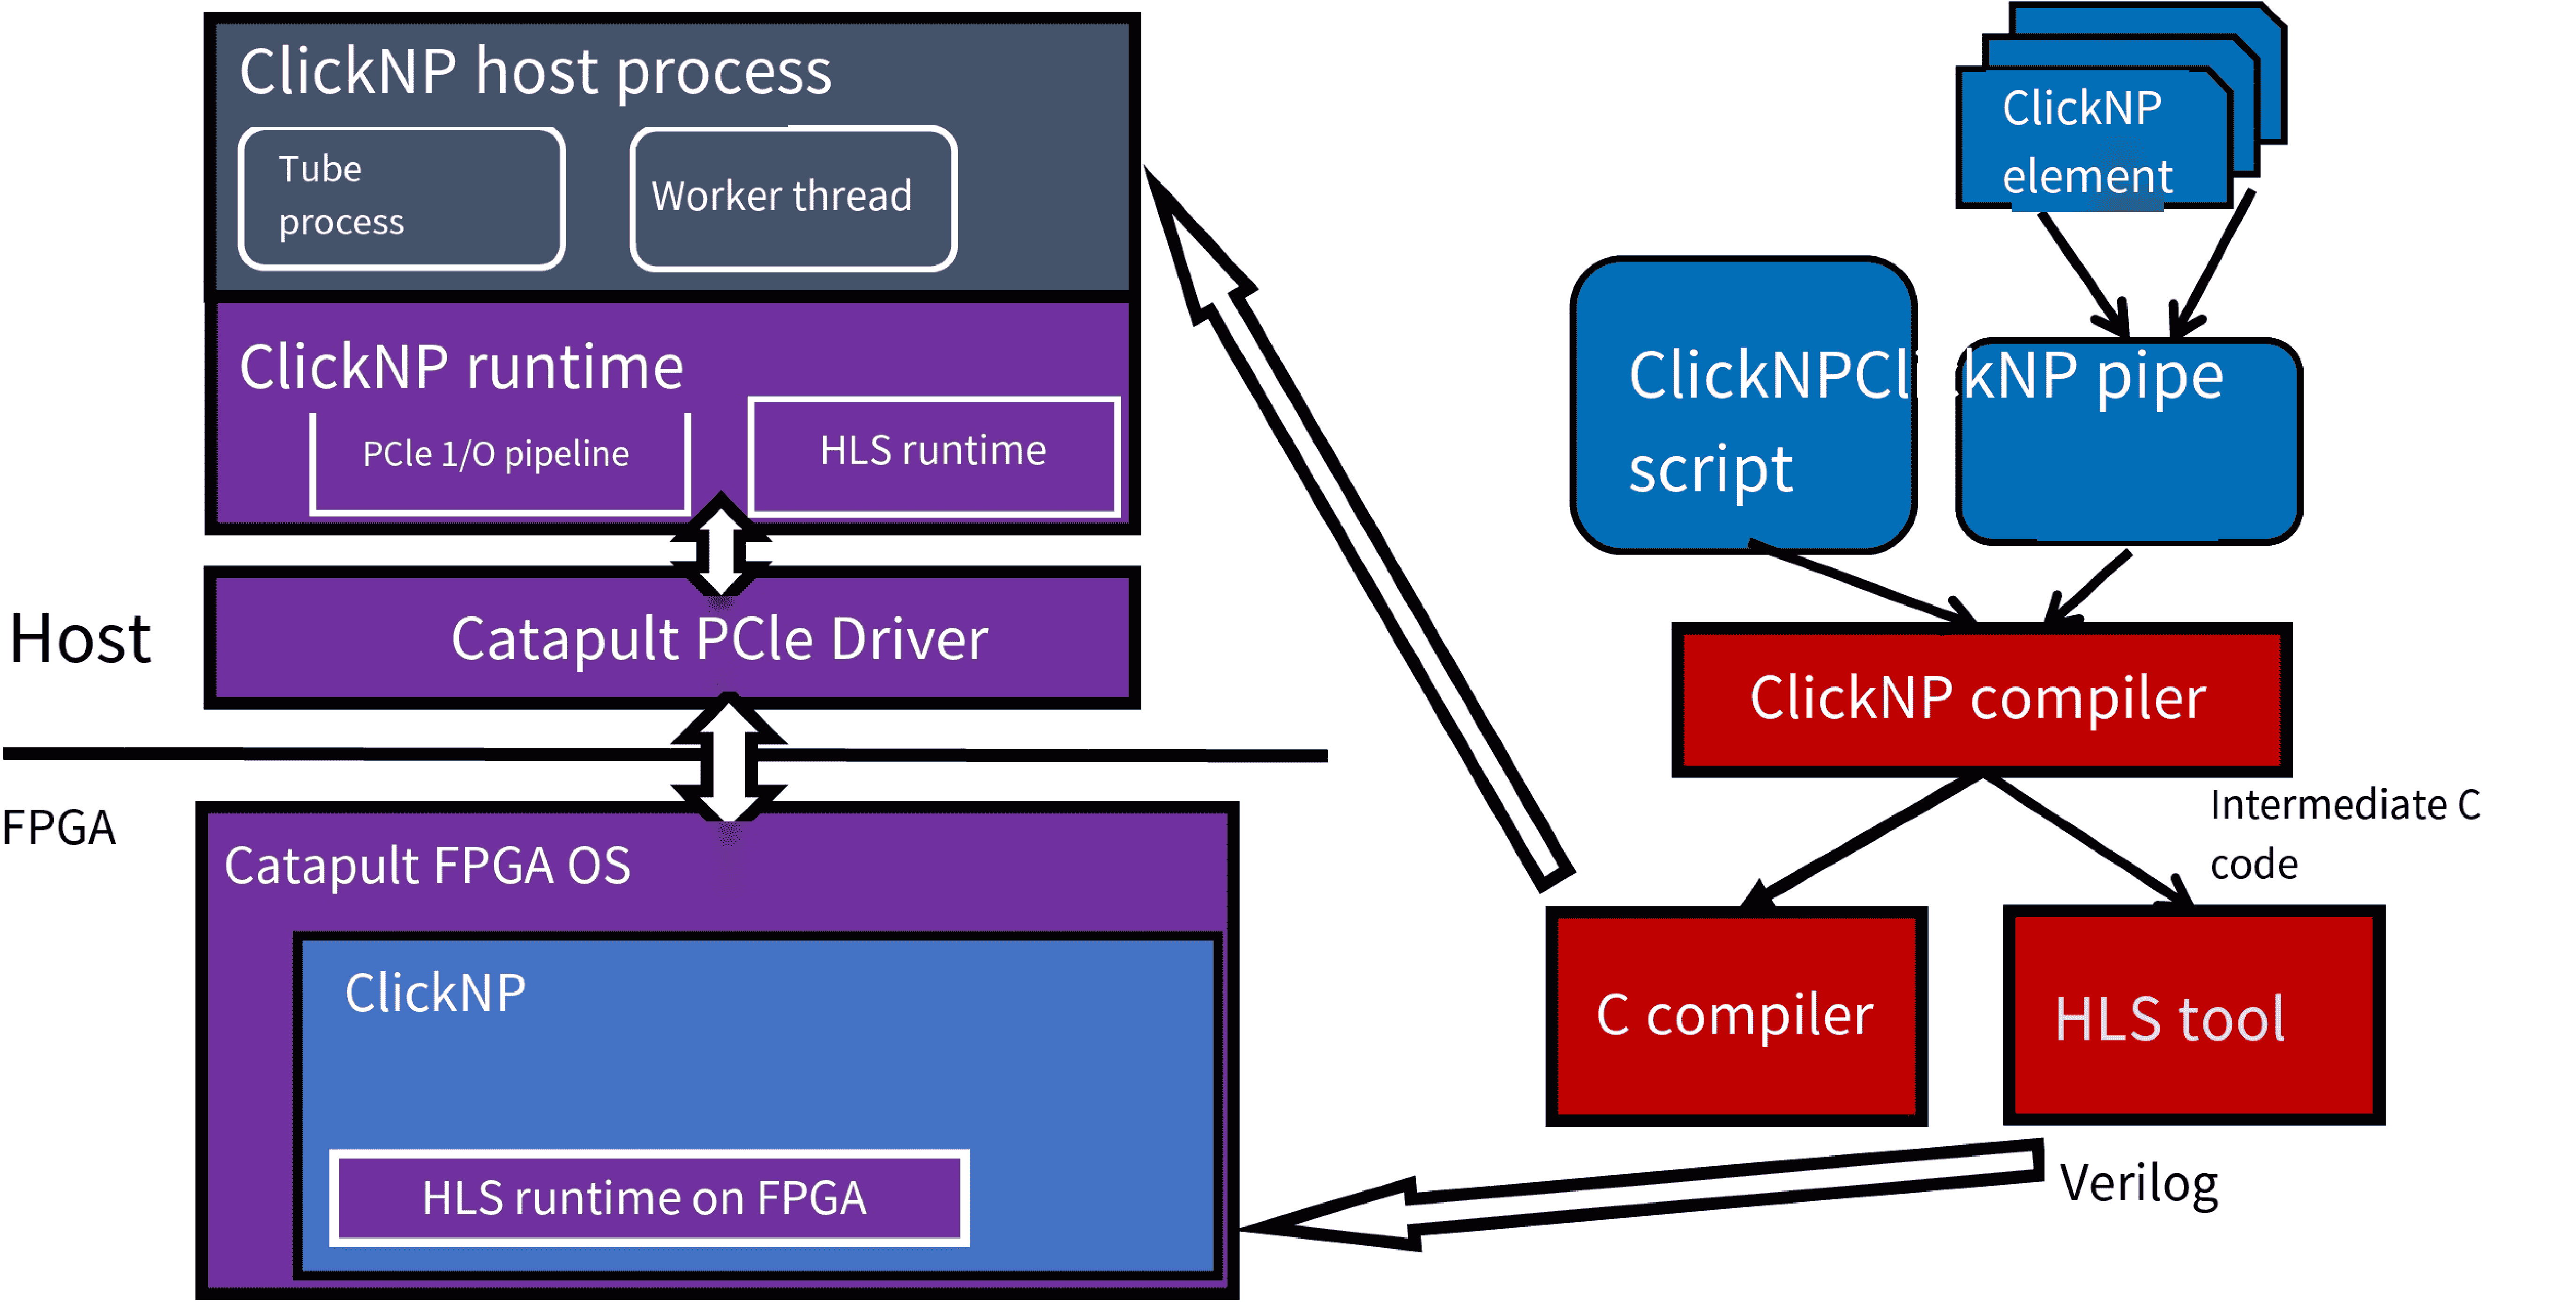
\includegraphics[width=.8\textwidth]{clicknp_arch.pdf}
	\caption{ClickNP Architecture.}
	\label{clicknp:fig:clicknp}
\end{figure}


The \name{} host process communicates with the \name{} user logic through the \name{} runtime library, which further relies on the services in the Catapult PCIe driver to interact with the FPGA hardware.
The \name{} runtime library implements two important functions:
(1) It exposes a PCIe channel API to achieve high-speed and low-latency communication between the \name{} host process and the role;
(2) It calls several high-level synthesis-specific libraries to pass initial parameters to the modules in the role and control the start/stop/reset of these modules.
The \name{} host process has a manager thread and zero or more worker threads.
The manager thread loads the FPGA image into the hardware, starts the worker threads, initializes the \name components in the FPGA and CPU according to the configuration, and controls their behavior by sending \textit {signals} to the components at runtime.
If each worker thread is assigned to a CPU, each worker thread can handle one or more modules.

\subsection{\name Programming}

\subsubsection{Abstraction}

\name provides a modular architecture, where the basic processing module is known as an \textit{element}. As shown in Figure \ref{clicknp:fig:element_arch}, \name elements have the following features:
\begin{itemize}
\item Local state. Each element can create a set of local variables that can only be accessed within the element itself.
\item Input and output ports. Elements can have any number of input or output ports.
\item Handler functions. Elements have three handler functions: (1) initialization handler, invoked once when the element starts, (2) processing handler, continuously called to inspect the input ports and process available data, and (3) signal handler, which receives and processes commands (\textit {signals}) from the manager thread in the host program.
\end{itemize}

\begin{figure}[htbp]
\centering
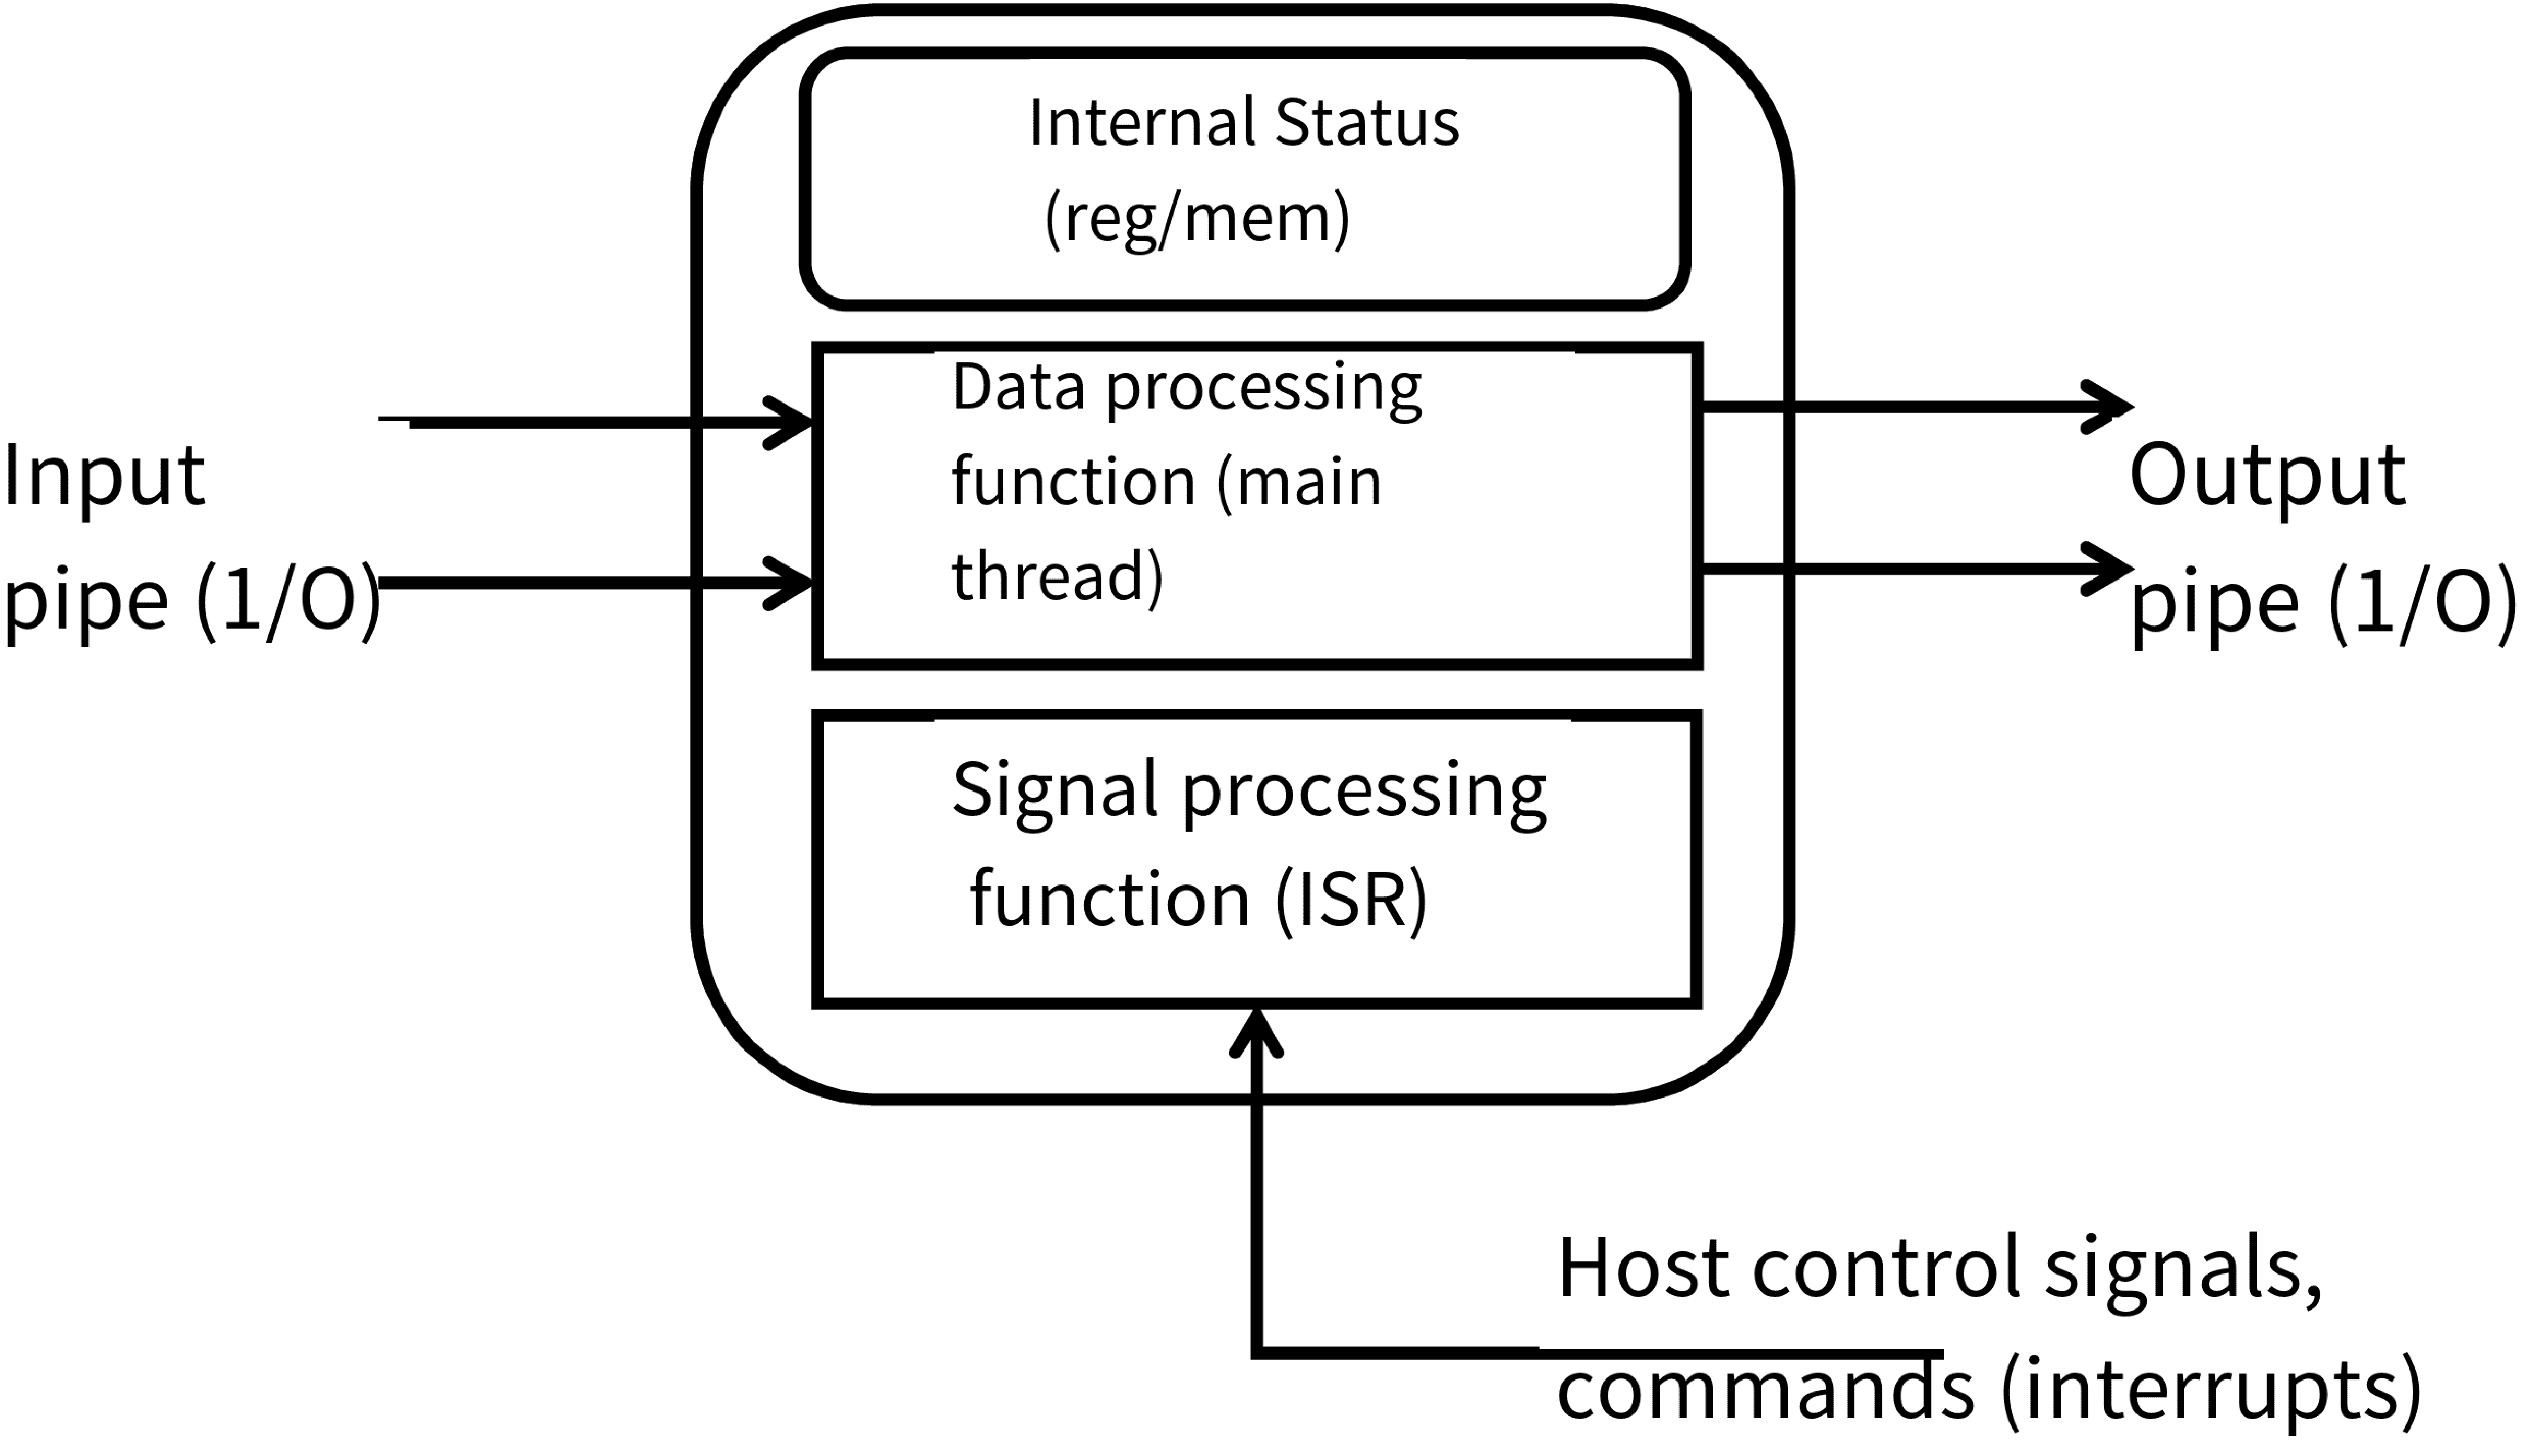
\includegraphics[width=.6\textwidth]{element_arch.pdf}
\caption{Composition of ClickNP elements.}
\label{clicknp:fig:element_arch}
\end{figure}

The output port of an element can be connected to the input port of another element through a \textit {channel}, as depicted in Figure \ref {clicknp:fig:element} (a). In \name, a channel is essentially a FIFO buffer, written at one end and read from the other. The data unit of read/write operations on the channel is known as a \textit {flit}, which has a fixed size of 64 bytes. The format of a flit is shown in Figure \ref {clicknp:fig:element} (b). Each flit contains a header of metadata and a payload of 32 bytes. When moving between \name elements, large amounts of data (e.g., full-size packets) are divided into multiple flits. The first flit is marked with \textbf {sop} (start of packet), and the last flit is marked with \textbf {eop} (end of packet). If the size of the data block is not 32, the \textbf {pad} field of the last flit indicates the number of bytes filled into the payload. The reserved fields in the flit have been optimized by the hardware description language synthesis tool. Dividing large data into flits not only reduces latency but also allows different segments of a packet to be processed simultaneously at different elements, increasing parallelism. Finally, to implement network functions, multiple \name elements can be interconnected to form a directed processing graph, known as a \name \textit {configuration}.

\begin{figure}[htbp]
	\centering
	\begin{tabular}{c}
		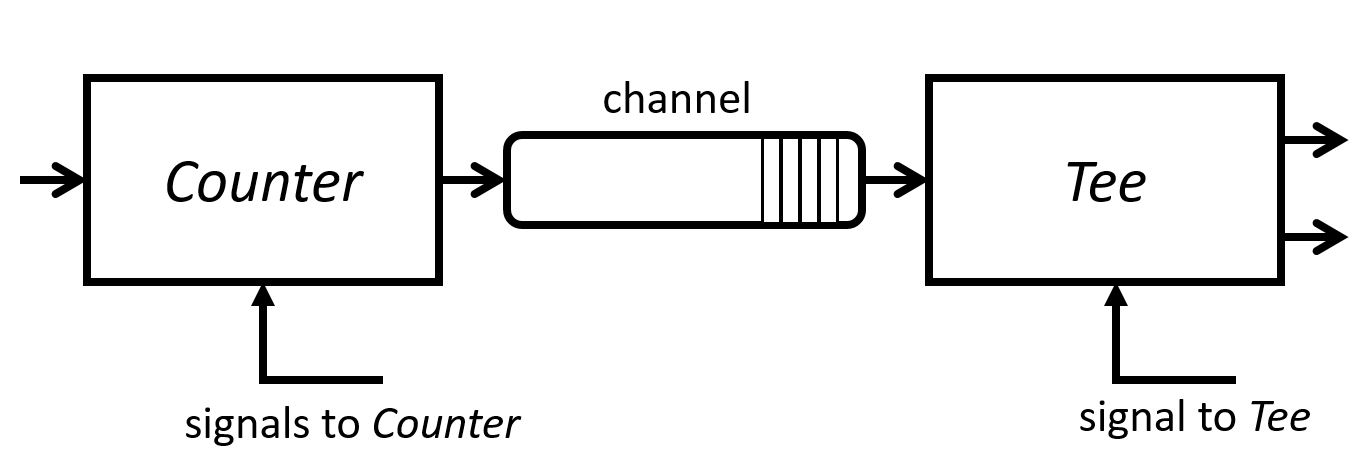
\includegraphics[width=.7\textwidth]{element.jpg}  \\
		(a)\\
		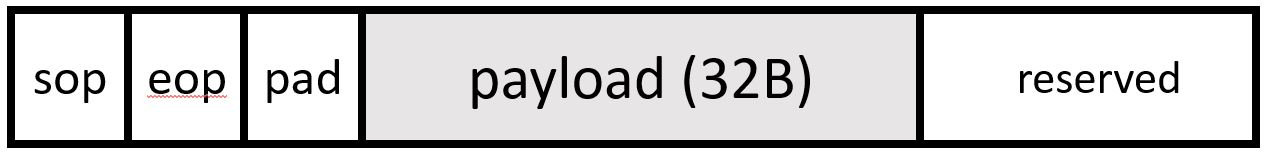
\includegraphics[width=.6\textwidth]{flit.jpg} \\
		(b) \\
	\end{tabular}
	\caption{(a) Two \name elements connected by a pipeline. (b) The format of Flit.}
	\label{clicknp:fig:element}
\end{figure}

Obviously, the \name programming abstraction is similar to the Click software router \cite {kohler2000click}.
However, there are three fundamental differences that make \name more suitable for FPGA implementation:
(1) In Click, the edges between elements are C++ function calls, and a \textit {queue} element is needed to store packets.
But in \name, the edges actually represent FIFO buffers that can hold actual data. Moreover, \name pipelines can break data dependencies between elements and allow them to run in parallel.
(2) Unlike Click, where each input/output port can \textit {write (push) or read (pull)} data, \name has unified these operations: an element can only \textit {write (push)} to the output port, and the input port can only perform \textit {read (pull)} operations.
(3) Click allows elements to directly call the methods of another element (through the context of a stream-based router), in \name, coordination between elements is \textit {message-based}, for example, the requester sends a request message to the responder and gets a response through another message.
Compared with coordination through shared memory, message-based coordination allows more parallelism and is more efficient in FPGAs, because access to shared memory can become a bottleneck.

\subsubsection{Language}

\name elements can be declared as an object in an object-oriented language (such as C++).
Unfortunately, many existing high-level synthesis tools only support the C language.
To take advantage of commercial high-level synthesis tools, a compiler can be written to convert an object-oriented language (such as C++) to C, but this effort is not easy.
This paper proposes a domain-specific language (DSL) based on a subset of the C language to support element declarations.

The translation of your LaTeX content is as follows:

\begin{figure}[htbp]
\lstset{ emph={%
		element, init, state, handler, signal,include
	}, emphstyle={\bfseries .},
	morekeywords={test_input_port,get_input_port,read_input_port,from_tor, to_tor, set_output_port, host, set_signal} 
}
\small
\centering
\begin{tabular}{c}
\begin{lstlisting}
element Count (flit in -> flit out) {
  state {
    ulong count;
  }
  init {
    count = 0;
  }
  handler {
    if (test_input_port(in)) {
      flit x;
      x = read_input_port(in);
      if (x.flit.fd.sop)
        count = count + 1;
      set_output_port(out, x);
    }
  }
  signal {
    ClSignal p;
    p.Sig.LParam[0] = count;
    set_signal(p);
  }
}
\end{lstlisting}
\end{tabular}
	\caption{Code of the packet counter element.}
	\label{clicknp:fig:count-element}
\end{figure}

Figure \ref{clicknp:fig:count-element} displays a code snippet of the \textit {Counter} element, which solely counts the number of packets that have passed through. The element is defined by the \textbf {.element} keyword, followed by the element name and input/output port declarations.
The \textbf {.state} keyword defines the state variables of the element, and \textbf {.init}, \textbf {.handler}, and \textbf {.signal} specify the initialization, data processing, and signal processing function elements.
Table \ref {clicknp:tab:built-in} enumerates the built-in functions for operating on input and output ports.

\begin{table}
	\centering
	\caption{Built-in operations on \name\ pipelines.}
	\label{clicknp:tab:built-in}
	\small
	\begin{tabular}{p{.4\textwidth}|p{.5\textwidth}}
		\toprule
		uint get\_input\_port() & Acquire a bitmap of all input ports with available data. \\
		\midrule
		bool test\_input\_port(uint id) & Test the input port indicated by id. \\
		\midrule
		flit read\_input\_port(uint id) & Read the input port indicated by id. \\
		\midrule
		flit peek\_input\_port(uint id) & Retrieve the data of the input port indicated by id, but do not remove it. \\
		\midrule
		void set\_output\_port(uint id, flit x) & Set flit as the output port. Upon the handler's return, flit will be written to the pipeline.\\
		\midrule
		ClSignal read\_signal() & Read the signal from the signal port.\\
		\midrule
		void set\_signal(ClSignal p) & Set the output signal on the signal port.\\
		\midrule
		return (uint bitmap) & The return value of \textbf{.handler} specifies the bitmap of the input ports to be read in the next iteration. \\
		\bottomrule
	\end{tabular}
\end{table}

Similar to Click, \name also utilizes simple scripts to specify the configuration of network functions, as depicted in Figure \ref{clicknp:fig:logger-config}. The configuration comprises two parts: \textit {declaration} and \textit {connection}, adhering to a syntax akin to the Click language \cite {kohler2000click}.
It is noteworthy that in \name, the keyword \textbf {host} can be employed to annotate elements, which will result in the elements being compiled into CPU binary files and executed on the CPU.

For elements that some high-level synthesis tools struggle to generate efficient hardware logic for, \name supports Verilog elements written in hardware description language. To integrate Verilog elements into the system, developers are required to write an element with the same interface as a placeholder (or a high-level language element with the same function for CPU debugging and testing), and declare it in the \name configuration file with the \textbf{verilog} keyword. The compilation toolchain will replace the Verilog module generated by the high-level synthesis tool for the placeholder element with the developer's implementation.

\begin{figure}[htbp]
\lstset{ emph={%
		element, init, state, handler, signal,include
	}, emphstyle={\bfseries .},
	morekeywords={get_input_port,read_input_port,from_tor, to_tor, set_output_port, host, set_signal} 
}
\small
\centering
\begin{tabular}{c}
\begin{lstlisting}
Count :: cnt @ 
Tee :: tee 
host PktLogger :: logger

from_tor -> cnt -> tee [1] -> to_tor
tee [2] -> logger
\end{lstlisting}
\end{tabular}
	\caption{The \name configuration file for the interconnection of packet capture tool elements. Elements annotated with the \textbf {host} keyword are compiled and executed on the CPU. Elements annotated with ``@'' need to receive control signals from the manager thread. \textbf {``From\_tor''} and \textbf {``to\_tor''} are two built-in elements, representing the input and output of the Ethernet port on the FPGA.}
	\label{clicknp:fig:logger-config}
\end{figure}

\iffalse
\begin{figure}[!t]
	\centering
	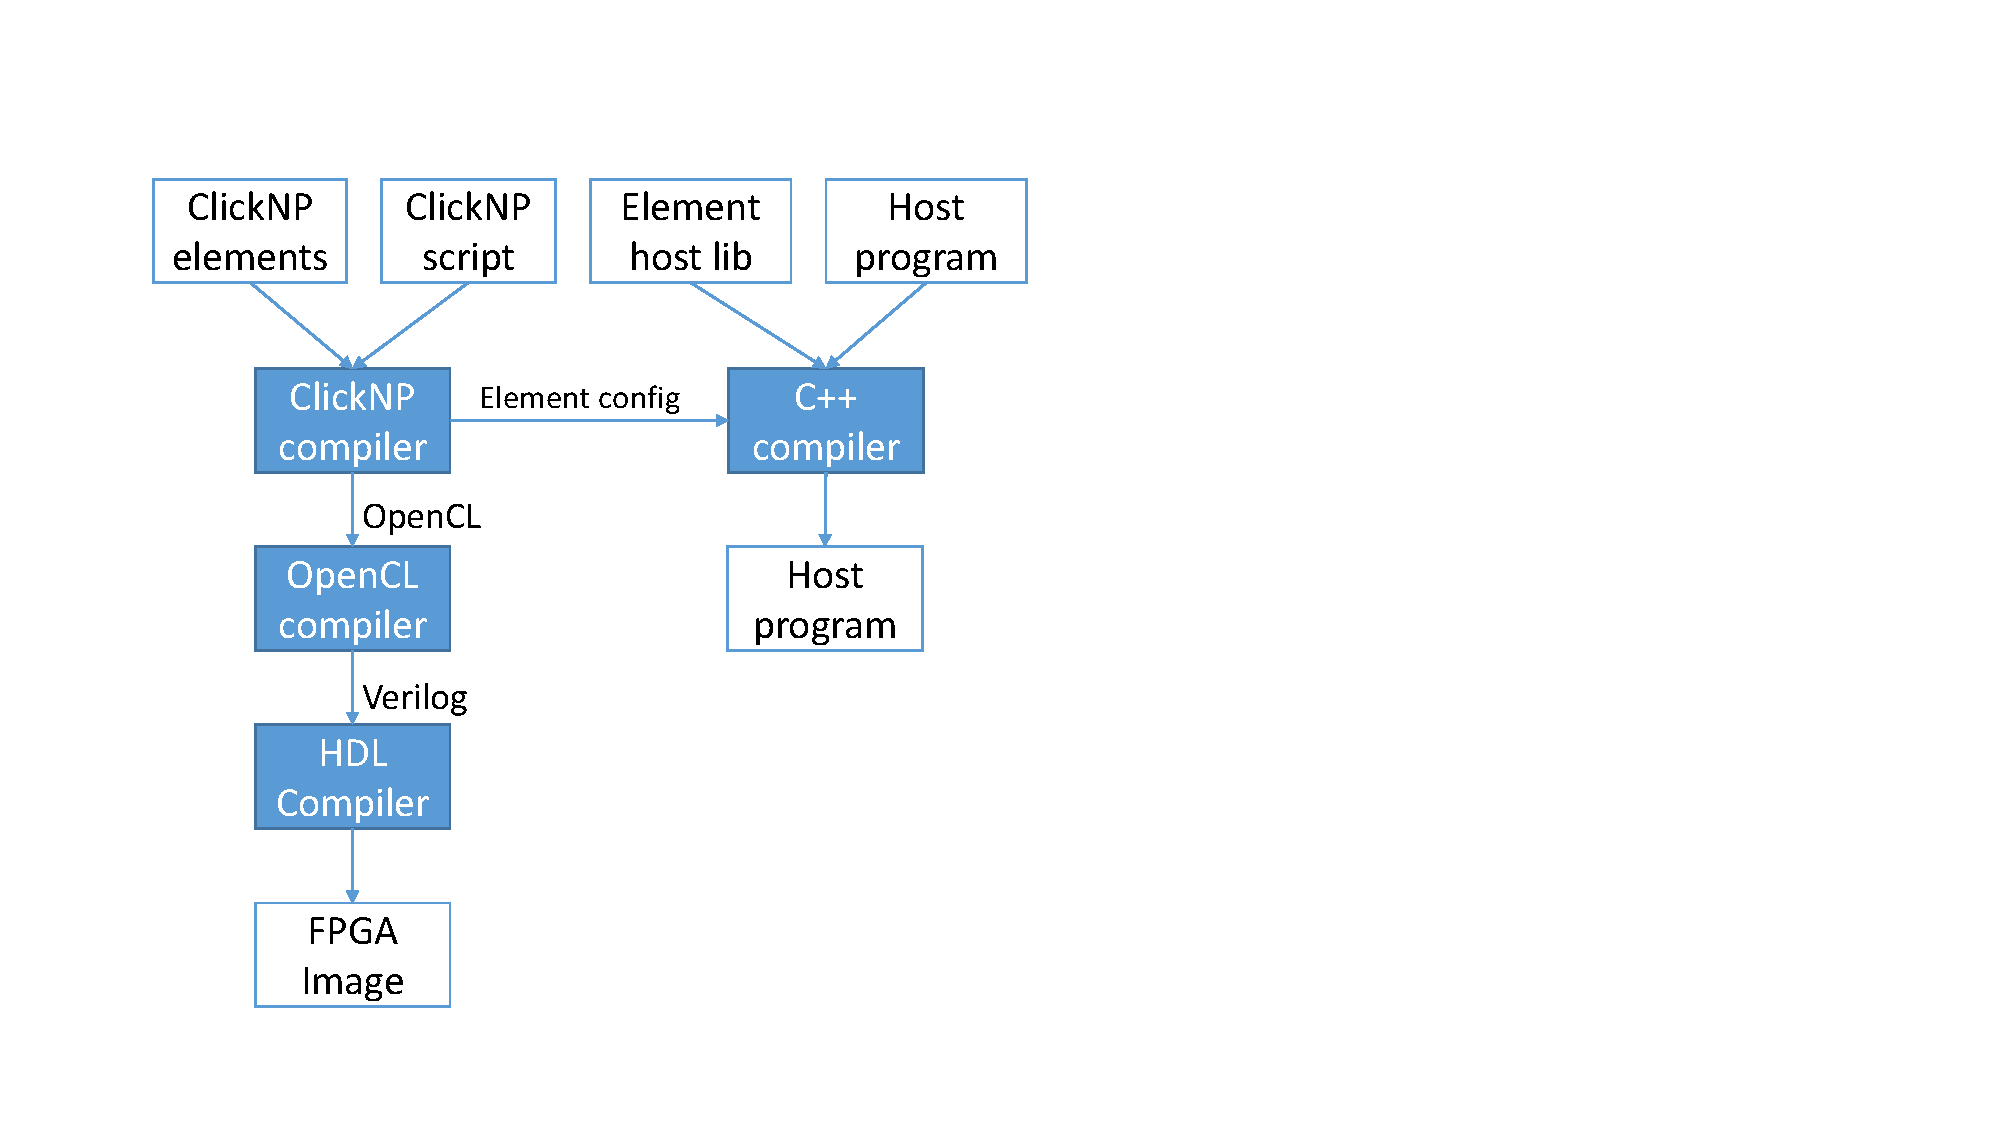
\includegraphics[width=0.8\columnwidth]{image/ClickNPSoftware}
	\vspace{-0.15in}
	\caption{ClickNP Compilation Flow}
	\vspace{-0.15in}
	\label{clicknp:fig:ClickNPSoftware}
	%    
\end{figure}

A comprehensive compilation of a project yields an FPGA image, an x86 host program, and an OpenCL kernel binary. Initially, the FPGA image is reprogrammed into the FPGA via the Flash Util as depicted in Figure \ref{clicknp:fig:CatapultFPGAArch} (30 seconds). Subsequently, the host program initiates, resets the FPGA board, loads the OpenCL kernel binary, and launches all kernels. The host program then proceeds to run, accepting control plane commands via the terminal or RPC, issuing signals to elements, and listening to events from elements.

When there is a requirement to update the host program, simply terminate the host program and the data plane will continue to function. The new host program can opt to either re-initialize all element states, or preserve the states and clear in-flight signals and events in the event that the host program was terminated midway through host-kernel communication.

\begin{figure}[!t]
	\centering
	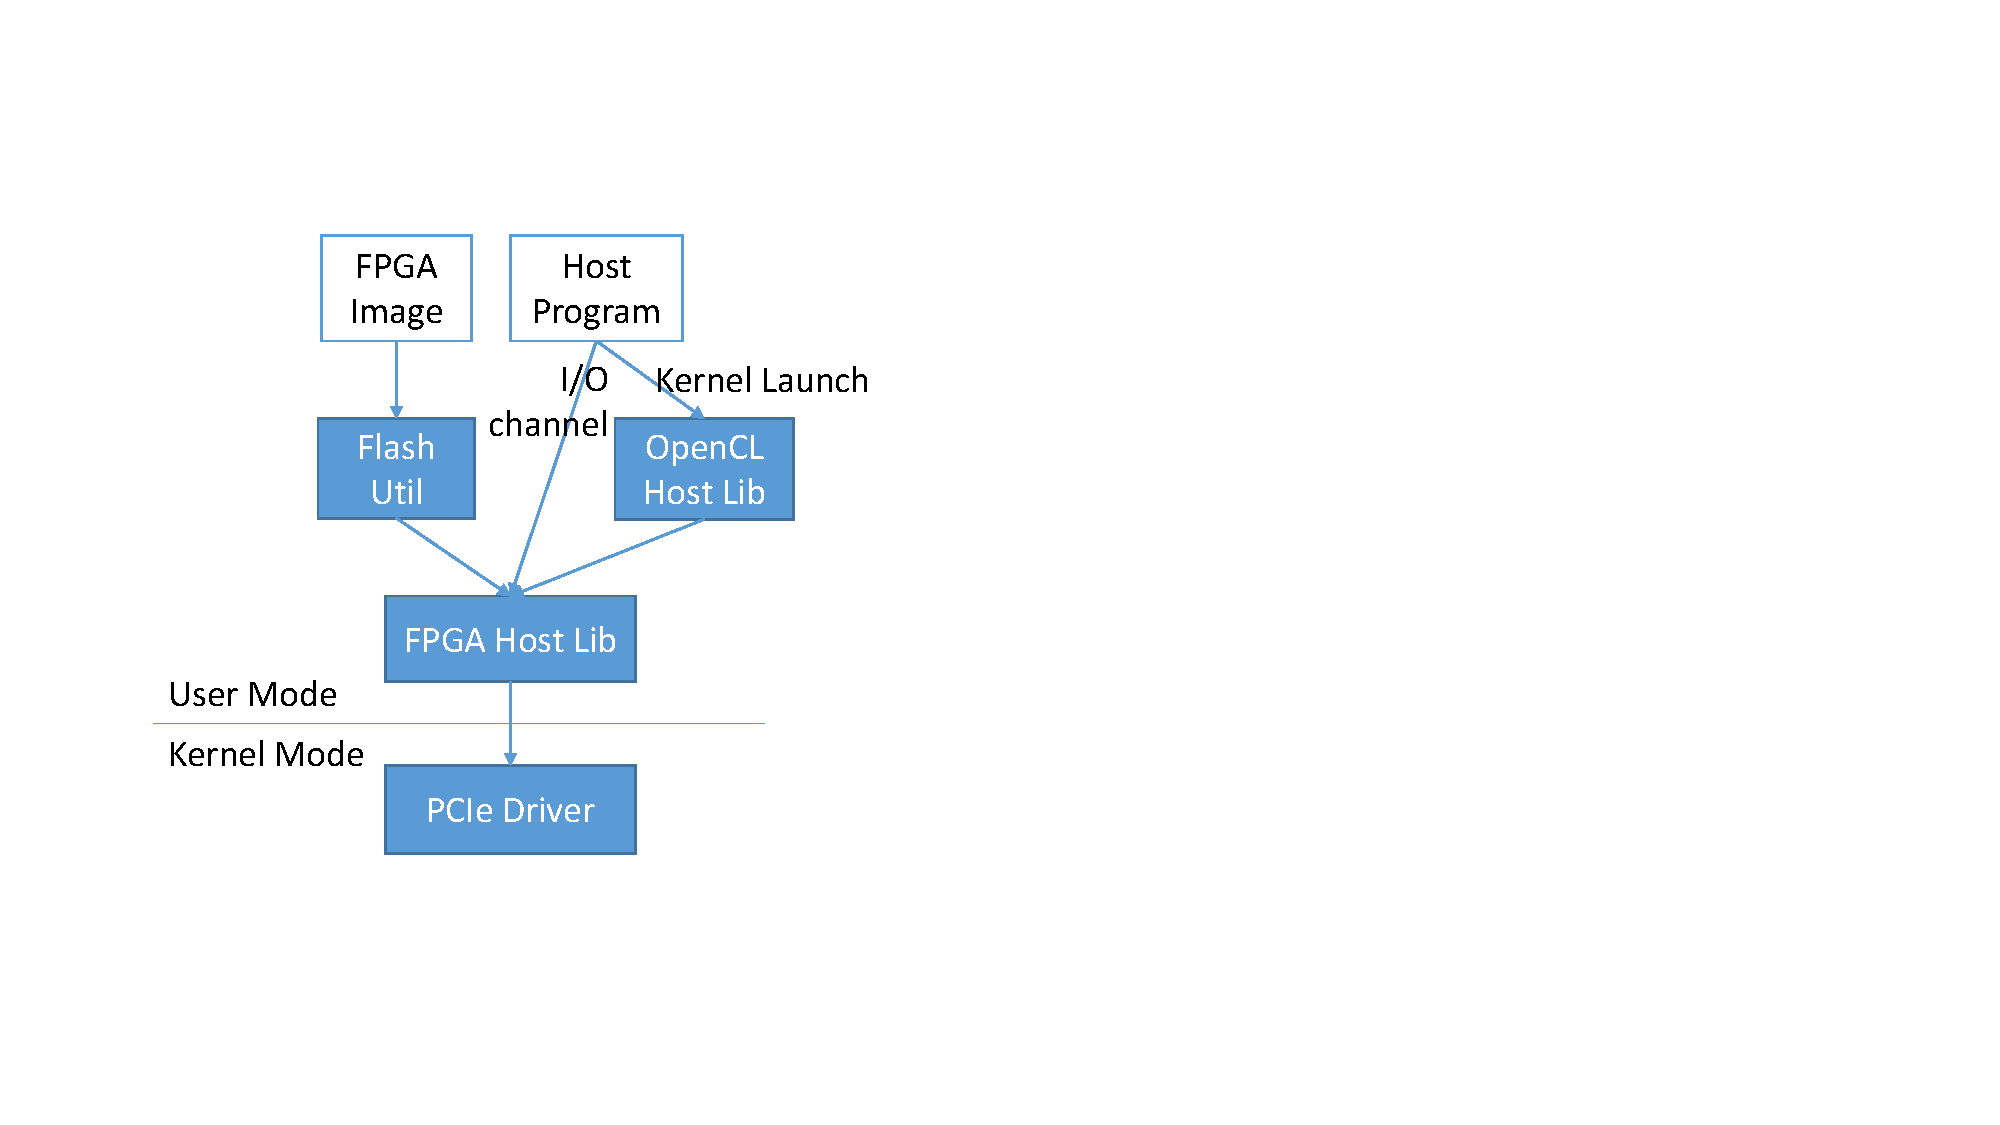
\includegraphics[width=0.8\columnwidth]{image/CatapultRuntime}
	\vspace{-0.15in}
	\caption{ClickNP Runtime Architecture}
	\vspace{-0.15in}
	\label{clicknp:fig:CatapultFPGAArch}
	%    
\end{figure}
\fi
